\hypertarget{h17block_8cpp}{}\section{h17block.\+cpp File Reference}
\label{h17block_8cpp}\index{h17block.\+cpp@{h17block.\+cpp}}
{\ttfamily \#include \char`\"{}h17block.\+h\char`\"{}}\\*
{\ttfamily \#include \char`\"{}track.\+h\char`\"{}}\\*
{\ttfamily \#include \char`\"{}sector.\+h\char`\"{}}\\*
{\ttfamily \#include \char`\"{}raw\+\_\+track.\+h\char`\"{}}\\*
{\ttfamily \#include \char`\"{}raw\+\_\+sector.\+h\char`\"{}}\\*
{\ttfamily \#include \char`\"{}dump.\+h\char`\"{}}\\*
{\ttfamily \#include $<$cstring$>$}\\*
Include dependency graph for h17block.\+cpp\+:\nopagebreak
\begin{figure}[H]
\begin{center}
\leavevmode
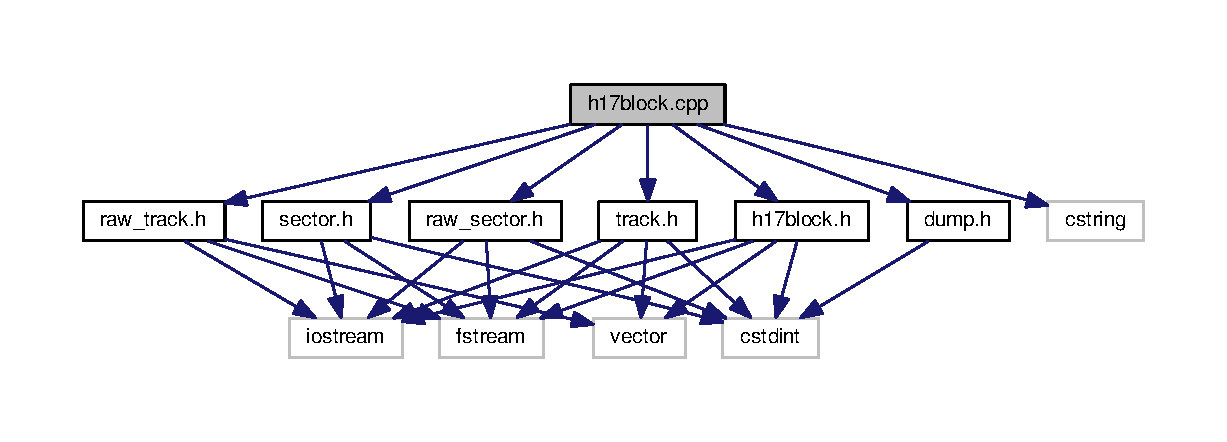
\includegraphics[width=350pt]{h17block_8cpp__incl}
\end{center}
\end{figure}


\subsection{Detailed Description}
Classes to handle the various blocks in the h17disk image file. 